\documentclass[]{article}
\usepackage{lmodern}
\usepackage{amssymb,amsmath}
\usepackage{ifxetex,ifluatex}
\usepackage{fixltx2e} % provides \textsubscript
\ifnum 0\ifxetex 1\fi\ifluatex 1\fi=0 % if pdftex
  \usepackage[T1]{fontenc}
  \usepackage[utf8]{inputenc}
\else % if luatex or xelatex
  \ifxetex
    \usepackage{mathspec}
  \else
    \usepackage{fontspec}
  \fi
  \defaultfontfeatures{Ligatures=TeX,Scale=MatchLowercase}
\fi
% use upquote if available, for straight quotes in verbatim environments
\IfFileExists{upquote.sty}{\usepackage{upquote}}{}
% use microtype if available
\IfFileExists{microtype.sty}{%
\usepackage{microtype}
\UseMicrotypeSet[protrusion]{basicmath} % disable protrusion for tt fonts
}{}
\usepackage[margin=1in]{geometry}
\usepackage{hyperref}
\hypersetup{unicode=true,
            pdftitle={Module 5: RESAMPLING},
            pdfauthor={Mette Langaas, Department of Mathematical Sciences, NTNU},
            pdfborder={0 0 0},
            breaklinks=true}
\urlstyle{same}  % don't use monospace font for urls
\usepackage{color}
\usepackage{fancyvrb}
\newcommand{\VerbBar}{|}
\newcommand{\VERB}{\Verb[commandchars=\\\{\}]}
\DefineVerbatimEnvironment{Highlighting}{Verbatim}{commandchars=\\\{\}}
% Add ',fontsize=\small' for more characters per line
\usepackage{framed}
\definecolor{shadecolor}{RGB}{248,248,248}
\newenvironment{Shaded}{\begin{snugshade}}{\end{snugshade}}
\newcommand{\AlertTok}[1]{\textcolor[rgb]{0.94,0.16,0.16}{#1}}
\newcommand{\AnnotationTok}[1]{\textcolor[rgb]{0.56,0.35,0.01}{\textbf{\textit{#1}}}}
\newcommand{\AttributeTok}[1]{\textcolor[rgb]{0.77,0.63,0.00}{#1}}
\newcommand{\BaseNTok}[1]{\textcolor[rgb]{0.00,0.00,0.81}{#1}}
\newcommand{\BuiltInTok}[1]{#1}
\newcommand{\CharTok}[1]{\textcolor[rgb]{0.31,0.60,0.02}{#1}}
\newcommand{\CommentTok}[1]{\textcolor[rgb]{0.56,0.35,0.01}{\textit{#1}}}
\newcommand{\CommentVarTok}[1]{\textcolor[rgb]{0.56,0.35,0.01}{\textbf{\textit{#1}}}}
\newcommand{\ConstantTok}[1]{\textcolor[rgb]{0.00,0.00,0.00}{#1}}
\newcommand{\ControlFlowTok}[1]{\textcolor[rgb]{0.13,0.29,0.53}{\textbf{#1}}}
\newcommand{\DataTypeTok}[1]{\textcolor[rgb]{0.13,0.29,0.53}{#1}}
\newcommand{\DecValTok}[1]{\textcolor[rgb]{0.00,0.00,0.81}{#1}}
\newcommand{\DocumentationTok}[1]{\textcolor[rgb]{0.56,0.35,0.01}{\textbf{\textit{#1}}}}
\newcommand{\ErrorTok}[1]{\textcolor[rgb]{0.64,0.00,0.00}{\textbf{#1}}}
\newcommand{\ExtensionTok}[1]{#1}
\newcommand{\FloatTok}[1]{\textcolor[rgb]{0.00,0.00,0.81}{#1}}
\newcommand{\FunctionTok}[1]{\textcolor[rgb]{0.00,0.00,0.00}{#1}}
\newcommand{\ImportTok}[1]{#1}
\newcommand{\InformationTok}[1]{\textcolor[rgb]{0.56,0.35,0.01}{\textbf{\textit{#1}}}}
\newcommand{\KeywordTok}[1]{\textcolor[rgb]{0.13,0.29,0.53}{\textbf{#1}}}
\newcommand{\NormalTok}[1]{#1}
\newcommand{\OperatorTok}[1]{\textcolor[rgb]{0.81,0.36,0.00}{\textbf{#1}}}
\newcommand{\OtherTok}[1]{\textcolor[rgb]{0.56,0.35,0.01}{#1}}
\newcommand{\PreprocessorTok}[1]{\textcolor[rgb]{0.56,0.35,0.01}{\textit{#1}}}
\newcommand{\RegionMarkerTok}[1]{#1}
\newcommand{\SpecialCharTok}[1]{\textcolor[rgb]{0.00,0.00,0.00}{#1}}
\newcommand{\SpecialStringTok}[1]{\textcolor[rgb]{0.31,0.60,0.02}{#1}}
\newcommand{\StringTok}[1]{\textcolor[rgb]{0.31,0.60,0.02}{#1}}
\newcommand{\VariableTok}[1]{\textcolor[rgb]{0.00,0.00,0.00}{#1}}
\newcommand{\VerbatimStringTok}[1]{\textcolor[rgb]{0.31,0.60,0.02}{#1}}
\newcommand{\WarningTok}[1]{\textcolor[rgb]{0.56,0.35,0.01}{\textbf{\textit{#1}}}}
\usepackage{graphicx,grffile}
\makeatletter
\def\maxwidth{\ifdim\Gin@nat@width>\linewidth\linewidth\else\Gin@nat@width\fi}
\def\maxheight{\ifdim\Gin@nat@height>\textheight\textheight\else\Gin@nat@height\fi}
\makeatother
% Scale images if necessary, so that they will not overflow the page
% margins by default, and it is still possible to overwrite the defaults
% using explicit options in \includegraphics[width, height, ...]{}
\setkeys{Gin}{width=\maxwidth,height=\maxheight,keepaspectratio}
\IfFileExists{parskip.sty}{%
\usepackage{parskip}
}{% else
\setlength{\parindent}{0pt}
\setlength{\parskip}{6pt plus 2pt minus 1pt}
}
\setlength{\emergencystretch}{3em}  % prevent overfull lines
\providecommand{\tightlist}{%
  \setlength{\itemsep}{0pt}\setlength{\parskip}{0pt}}
\setcounter{secnumdepth}{0}
% Redefines (sub)paragraphs to behave more like sections
\ifx\paragraph\undefined\else
\let\oldparagraph\paragraph
\renewcommand{\paragraph}[1]{\oldparagraph{#1}\mbox{}}
\fi
\ifx\subparagraph\undefined\else
\let\oldsubparagraph\subparagraph
\renewcommand{\subparagraph}[1]{\oldsubparagraph{#1}\mbox{}}
\fi

%%% Use protect on footnotes to avoid problems with footnotes in titles
\let\rmarkdownfootnote\footnote%
\def\footnote{\protect\rmarkdownfootnote}

%%% Change title format to be more compact
\usepackage{titling}

% Create subtitle command for use in maketitle
\providecommand{\subtitle}[1]{
  \posttitle{
    \begin{center}\large#1\end{center}
    }
}

\setlength{\droptitle}{-2em}

  \title{Module 5: RESAMPLING}
    \pretitle{\vspace{\droptitle}\centering\huge}
  \posttitle{\par}
  \subtitle{TMA4268 Statistical Learning V2019}
  \author{Mette Langaas, Department of Mathematical Sciences, NTNU}
    \preauthor{\centering\large\emph}
  \postauthor{\par}
      \predate{\centering\large\emph}
  \postdate{\par}
    \date{week 6 2019}

\usepackage{booktabs}
\usepackage{makecell}

\begin{document}
\maketitle

{
\setcounter{tocdepth}{2}
\tableofcontents
}
Last changes: (05.02: added link to R Markdown intro, under Interactive
lecture. 04.02. added class notes with improved drawing for two layers
of CV)

\hypertarget{introduction}{%
\section{ Introduction}\label{introduction}}

\hypertarget{learning-material-for-this-module}{%
\subsection{Learning material for this
module}\label{learning-material-for-this-module}}

\begin{itemize}
\tightlist
\item
  James et al (2013): An Introduction to Statistical Learning. Chapter
  5.
\item
  \href{https://www.math.ntnu.no/emner/TMA4268/2019v/notes/M5L1notes.pdf}{Classnotes
  04.02.2019}
\end{itemize}

Additional material for the interested reader: Chapter 7 (in particular
7.10) in Friedman et al (2001): Elements of Statistical learning.

\hypertarget{move-to}{%
\subsection{Move to}\label{move-to}}

\begin{itemize}
\tightlist
\item
  \protect\hyperlink{intro}{Introduction}
\item
  \protect\hyperlink{cv}{Cross-validation} and
  \protect\hyperlink{recexcv}{Recommended exercises on cross-validation}
\item
  \protect\hyperlink{boot}{Bootstrapping} and
  \protect\hyperlink{recexboot}{Recommended exercises on bootstrapping}
\item
  \protect\hyperlink{summing}{Summing up}
\item
  \protect\hyperlink{further}{Further reading}
\item
  \protect\hyperlink{Rpackages}{R packages}
\end{itemize}

\begin{center}\rule{0.5\linewidth}{\linethickness}\end{center}

\hypertarget{what-will-you-learn}{%
\subsection{What will you learn?}\label{what-will-you-learn}}

\begin{itemize}
\tightlist
\item
  What is model assessment and model selection?
\item
  Ideal solution in a data rich situation.
\item
  Cross-validation: validation set - LOOCV and \(k\)-fold CV - what is
  the best?
\item
  Bootstrapping - how and why.
\item
  Summing up
\item
  The plan for the interactive lesson.
\end{itemize}

\begin{center}\rule{0.5\linewidth}{\linethickness}\end{center}

\hypertarget{generalization-performance-of-learning-method}{%
\section{Generalization performance of learning
method}\label{generalization-performance-of-learning-method}}

\begin{itemize}
\tightlist
\item
  prediction capacity on independent test data
\item
  inference and understanding
\end{itemize}

This is important both for

\hypertarget{model-selection}{%
\subsubsection{Model selection}\label{model-selection}}

estimate the \emph{performance} of different models (often different
order of complexity within one model class) to \emph{choose the best
model}.

\hypertarget{model-assessment}{%
\subsubsection{Model assessment}\label{model-assessment}}

having chosen a final model, estimating its performance (prediction
error) on new data.

\begin{center}\rule{0.5\linewidth}{\linethickness}\end{center}

\hypertarget{example}{%
\subsubsection{Example}\label{example}}

We aim to do \emph{model selection} in KNN-regression, where true curve
is \(f(x)=-x+x^2+x^3\) with \(x \in [-3,3]\). \(n=61\) for the training
data.

\begin{figure}
\centering
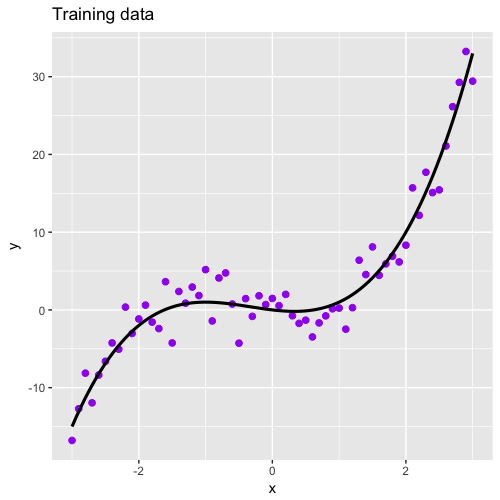
\includegraphics{Prob1f1.png}
\caption{Regression problem: training data and true regression curve}
\end{figure}

\begin{center}\rule{0.5\linewidth}{\linethickness}\end{center}

\hypertarget{knn-regression}{%
\subsubsection{KNN-regression}\label{knn-regression}}

\(n=61\) both for training and for test data (using same x-grid).

\begin{figure}
\centering
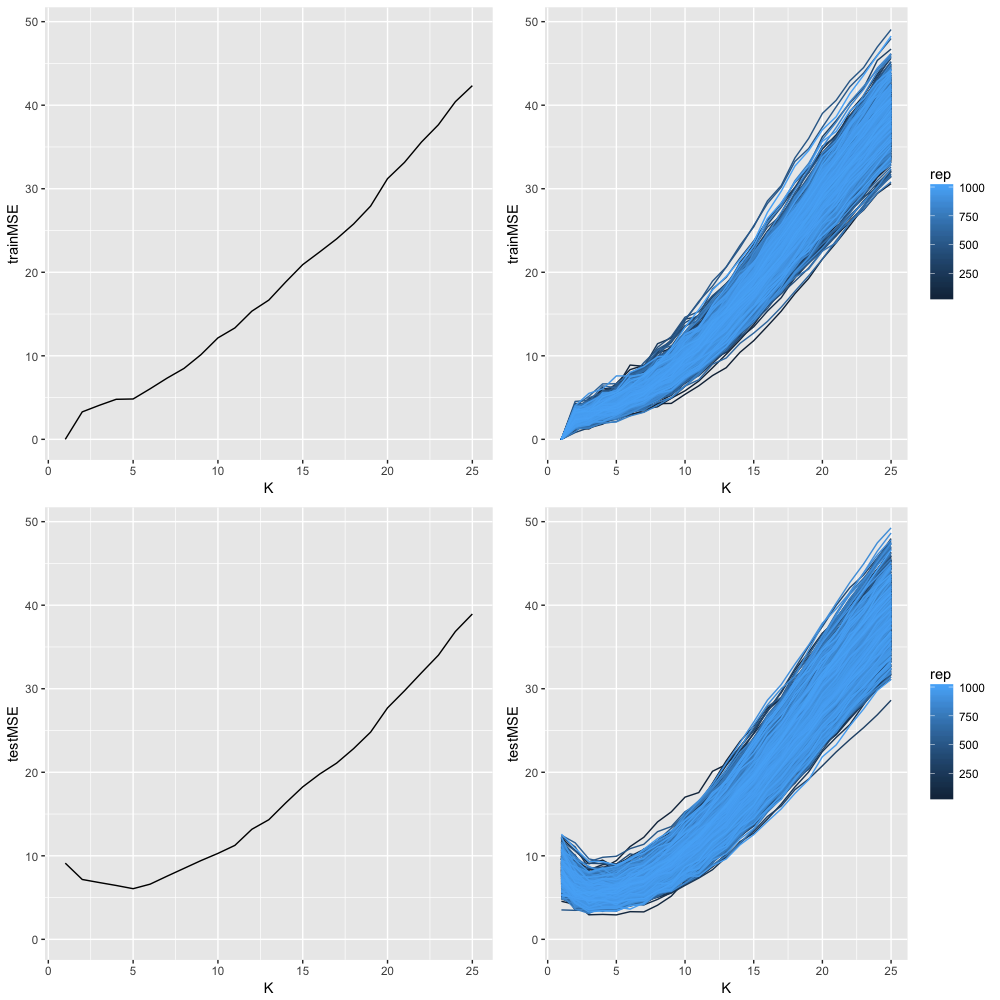
\includegraphics{Prob1f3.png}
\caption{Regression problem: MSE for training and test set, M=1000
versions}
\end{figure}

\(K\) small: high complexity (left) and \(K\) large: low complexity
(right).

Take home message: the training error rate is often very different from
the test error rate - and looking at the training error to estimate the
test error will dramatically underestimate the latter.

\begin{center}\rule{0.5\linewidth}{\linethickness}\end{center}

\hypertarget{the-bias-variance-trade-off}{%
\section{The bias-variance
trade-off}\label{the-bias-variance-trade-off}}

\begin{figure}
\centering
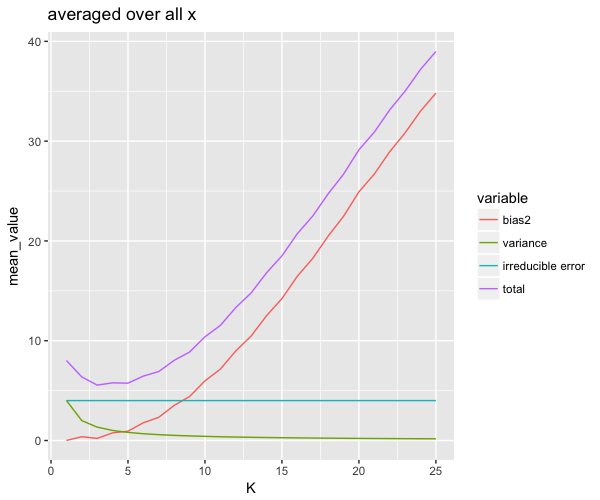
\includegraphics{Prob1f4.png}
\caption{Regression problem: bias-variance traceoff}
\end{figure}

Left (high complexity): low squared-bias (red) and high variance
(green). Right (low complexity): high squared-bias (red) and low
variance (green).

\begin{center}\rule{0.5\linewidth}{\linethickness}\end{center}

\hypertarget{loss-functions}{%
\subsection{Loss functions}\label{loss-functions}}

reminder - we will use

\begin{itemize}
\item
  Mean squared error (quadratic loss) for regression problems:
  \[Y_i=f({\bf x}_i)+\varepsilon_i \text{ for }i=1,\ldots,n \text{ and } \text{MSE}=\frac{1}{n}\sum_{i=1}^n (y_i-\hat{f}({\bf x}_i))^2\]
\item
  0/1 loss for classification problems:
  \[P(Y=j\mid {\bf x}_0) \text{ for }j=1,\ldots,K \] and classify to the
  class with the highest probability \(\hat{y}_i\). Then
  \[\frac{1}{n}\sum_{i=1}^n \text{I}(y_i \neq \hat{y}_i)\] will give the
  misclassification rate.
\end{itemize}

\begin{center}\rule{0.5\linewidth}{\linethickness}\end{center}

\hypertarget{the-challenge}{%
\subsubsection{The challenge}\label{the-challenge}}

our example was based on simulated data, so I had unlimited access to
data. Now, let us move to real data.

\begin{center}\rule{0.5\linewidth}{\linethickness}\end{center}

\hypertarget{data-rich-situation}{%
\section{Data rich situation}\label{data-rich-situation}}

If we had a large amount of data we could divide our data into three
parts:

\begin{itemize}
\tightlist
\item
  training set: to fit the model
\item
  validation set: to select the best model (aka model selection)
\item
  test set: to assess how well the model fits on new independent data
  (aka model assessment)
\end{itemize}

\textbf{Q}: Before we had just training and test. Why do we need the
additional validation set?

\textbf{A}: We have not discussed model selection before.

\textbf{Q}: Why can't we just use the training set for training, and
then the test set both for model selection and for model evaluation?

\textbf{A}: We will too optimistic if we report the error on the test
set when we have already used the test set to choose the best model.

\begin{center}\rule{0.5\linewidth}{\linethickness}\end{center}

If this is the case - great - then you do not need Module 5. But, this
is very seldom the case - so we will study other solutions based on
efficient sample reuse with \emph{resampling} data.

An alternative strategy for model selection (using methods penalizing
model complexity, e.g.~AIC or lasso) is covered in Module 6.

First we look at \emph{crossvalidation}, then at \emph{bootstrapping}.

\begin{center}\rule{0.5\linewidth}{\linethickness}\end{center}

\hypertarget{cross-validation-cv}{%
\section{Cross-validation (CV)}\label{cross-validation-cv}}

Consider the following ``model selection'' situation: We assume that
test data is available (and has been put aside), and we want to use the
rest of our data to both fit the data and to find the best model.

This can be done by:

\begin{itemize}
\tightlist
\item
  the validation set approach (what we have already looked at above)
\item
  leave one out cross validation (LOOCV)
\item
  5 and 10 fold crossvalidation (CV)
\end{itemize}

We will also discuss that there is a ``right and a wrong way'' to to CV

\begin{itemize}
\tightlist
\item
  selection bias - all elements of a model selection strategy need to be
  within the CV-loop
\item
  recommended exercises
\end{itemize}

\begin{center}\rule{0.5\linewidth}{\linethickness}\end{center}

\hypertarget{the-validation-set-approach}{%
\subsection{The validation set
approach}\label{the-validation-set-approach}}

Consider the case when you have a data set consisting of \(n\)
observations.

To fit a model and to evaluate its predictive performance you randomly
divide the data set into two parts (\(n/2\) sample size each):

\begin{itemize}
\tightlist
\item
  a \emph{training set} (to fit the model) and
\item
  a \emph{validation set} (to make predictions of the response variable
  for the observations in the validation set)
\end{itemize}

Remember: focus is on model selection (more in Module 6 - for example
how to perform model selection with linear regression). )

\begin{center}\rule{0.5\linewidth}{\linethickness}\end{center}

\hypertarget{regression-model-selection-example-validation-set-error}{%
\subsubsection{Regression model selection example: validation set
error}\label{regression-model-selection-example-validation-set-error}}

Auto data set (library \texttt{ISLR}): predict \texttt{mpg} (miles pr
gallon) using polynomial function of \texttt{horsepower} (of engine),
\(n=392\). What do you see?

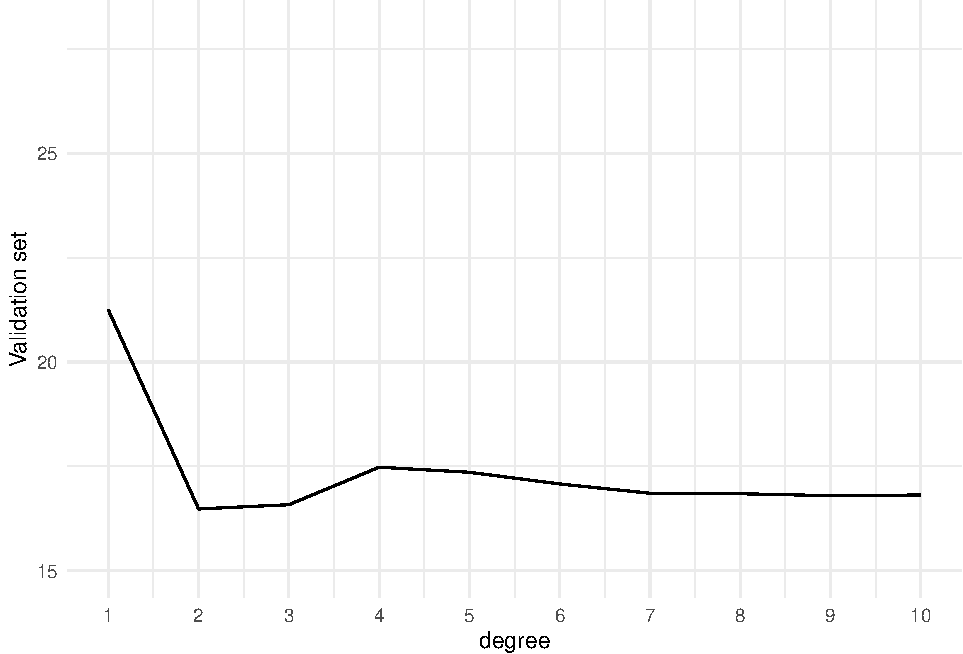
\includegraphics{5Resample_files/figure-latex/unnamed-chunk-1-1.pdf}

\begin{center}\rule{0.5\linewidth}{\linethickness}\end{center}

\hypertarget{regression-example-validation-set-error-for-many-random-divisions}{%
\subsubsection{Regression example: validation set error for many random
divisions}\label{regression-example-validation-set-error-for-many-random-divisions}}

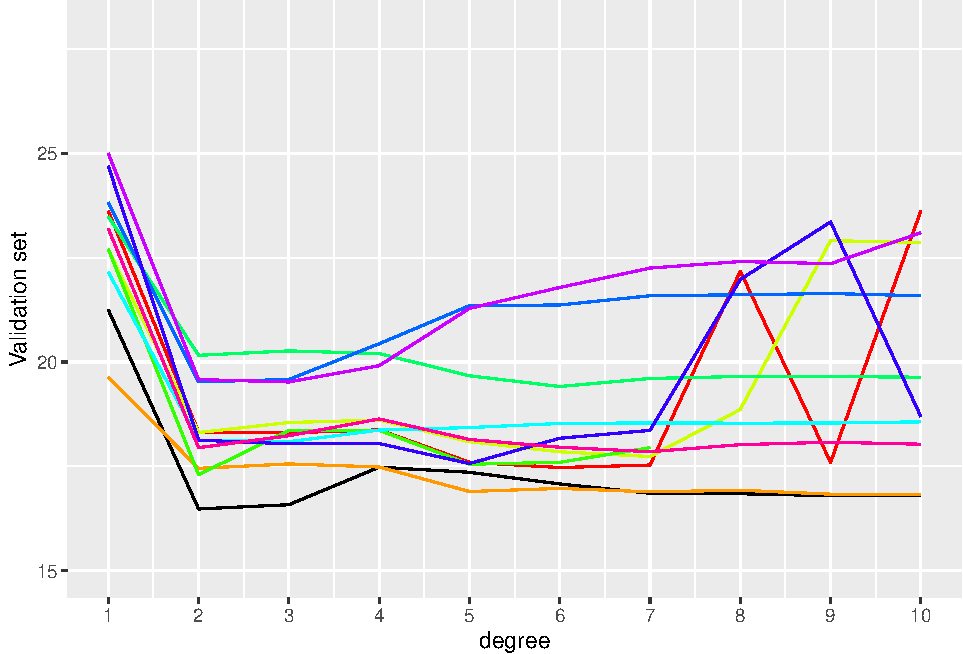
\includegraphics{5Resample_files/figure-latex/unnamed-chunk-2-1.pdf}

\begin{center}\rule{0.5\linewidth}{\linethickness}\end{center}

\hypertarget{drawbacks-with-the-validation-set-approach}{%
\subsubsection{Drawbacks with the validation set
approach}\label{drawbacks-with-the-validation-set-approach}}

\begin{itemize}
\tightlist
\item
  high variability of validation set error - since this is dependent on
  which observation are included in the training and validation set
\item
  smaller sample size for model fit - since not all observations can be
  in the training set
\item
  the validation set error may tend to overestimate the error rate on
  new observations for a model that is fit on the full data set (because
  - the more data the lower error, and here our training set is half of
  our data set).
\end{itemize}

\begin{center}\rule{0.5\linewidth}{\linethickness}\end{center}

\hypertarget{leave-one-out-cross-validation-loocv}{%
\subsection{Leave-one-out cross-validation
(LOOCV)}\label{leave-one-out-cross-validation-loocv}}

\begin{itemize}
\tightlist
\item
  If the data is very limited and the division of the data into two
  parts is unreasonable, leave-one-out cross-validation (LOOCV) can be
  used.
\item
  In LOOCV one observation at a time is left out and makes up the new
  observations (test set).
\item
  The remaining \(n-1\) observations make up the training set.
\item
  The procedure of model fitting is repeated \(n\) times, such that each
  of the \(n\) observations is left out once.
\item
  The total prediction error is the mean across these \(n\) models.
\end{itemize}

\[\text{MSE}_i=(y_i-\hat{y}_i)^2\]

\[CV_{n}=\frac{1}{n}\sum_{i=1}^n \text{MSE}_i\]

\begin{center}\rule{0.5\linewidth}{\linethickness}\end{center}

\hypertarget{regression-example-loocv}{%
\subsubsection{Regression example:
LOOCV}\label{regression-example-loocv}}

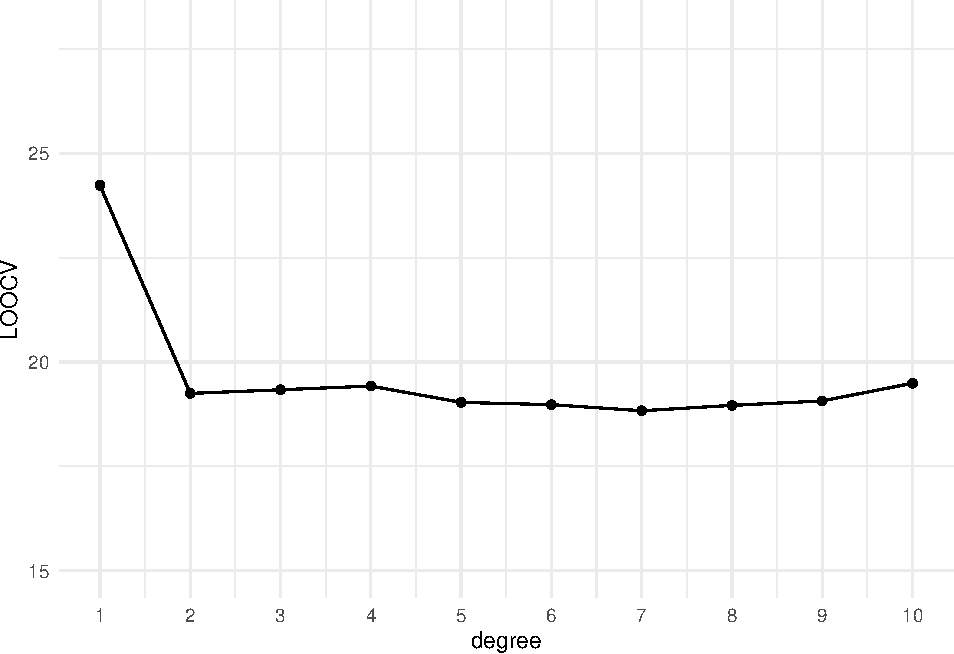
\includegraphics{5Resample_files/figure-latex/unnamed-chunk-3-1.pdf}

\begin{center}\rule{0.5\linewidth}{\linethickness}\end{center}

\tiny

\begin{Shaded}
\begin{Highlighting}[]
\KeywordTok{library}\NormalTok{(ISLR)  }\CommentTok{#for Auto data set}
\KeywordTok{library}\NormalTok{(boot)  }\CommentTok{#for cv.glm}
\KeywordTok{library}\NormalTok{(ggplot2)  }\CommentTok{#for plotting}
\KeywordTok{set.seed}\NormalTok{(}\DecValTok{123}\NormalTok{)}
\NormalTok{n =}\StringTok{ }\KeywordTok{dim}\NormalTok{(Auto)[}\DecValTok{1}\NormalTok{]}
\NormalTok{testMSEvec =}\StringTok{ }\OtherTok{NULL}
\NormalTok{start =}\StringTok{ }\KeywordTok{Sys.time}\NormalTok{()}
\ControlFlowTok{for}\NormalTok{ (polydeg }\ControlFlowTok{in} \DecValTok{1}\OperatorTok{:}\DecValTok{10}\NormalTok{) \{}
\NormalTok{    glm.fit =}\StringTok{ }\KeywordTok{glm}\NormalTok{(mpg }\OperatorTok{~}\StringTok{ }\KeywordTok{poly}\NormalTok{(horsepower, polydeg), }\DataTypeTok{data =}\NormalTok{ Auto)}
\NormalTok{    glm.cv1 =}\StringTok{ }\KeywordTok{cv.glm}\NormalTok{(Auto, glm.fit, }\DataTypeTok{K =}\NormalTok{ n)}
\NormalTok{    testMSEvec =}\StringTok{ }\KeywordTok{c}\NormalTok{(testMSEvec, glm.cv1}\OperatorTok{$}\NormalTok{delta[}\DecValTok{1}\NormalTok{])}
\NormalTok{\}}
\NormalTok{stopp =}\StringTok{ }\KeywordTok{Sys.time}\NormalTok{()}
\NormalTok{yrange =}\StringTok{ }\KeywordTok{c}\NormalTok{(}\DecValTok{15}\NormalTok{, }\DecValTok{28}\NormalTok{)}
\NormalTok{plotdf =}\StringTok{ }\KeywordTok{data.frame}\NormalTok{(}\DataTypeTok{testMSE =}\NormalTok{ testMSEvec, }\DataTypeTok{degree =} \DecValTok{1}\OperatorTok{:}\DecValTok{10}\NormalTok{)}
\NormalTok{g0 =}\StringTok{ }\KeywordTok{ggplot}\NormalTok{(plotdf, }\KeywordTok{aes}\NormalTok{(}\DataTypeTok{x =}\NormalTok{ degree, }\DataTypeTok{y =}\NormalTok{ testMSE)) }\OperatorTok{+}\StringTok{ }\KeywordTok{geom_line}\NormalTok{() }\OperatorTok{+}\StringTok{ }\KeywordTok{geom_point}\NormalTok{() }\OperatorTok{+}\StringTok{ }
\StringTok{    }\KeywordTok{scale_y_continuous}\NormalTok{(}\DataTypeTok{limits =}\NormalTok{ yrange) }\OperatorTok{+}\StringTok{ }\KeywordTok{scale_x_continuous}\NormalTok{(}\DataTypeTok{breaks =} \DecValTok{1}\OperatorTok{:}\DecValTok{10}\NormalTok{) }\OperatorTok{+}\StringTok{ }
\StringTok{    }\KeywordTok{labs}\NormalTok{(}\DataTypeTok{y =} \StringTok{"LOOCV"}\NormalTok{)}
\NormalTok{g0 }\OperatorTok{+}\StringTok{ }\KeywordTok{theme_minimal}\NormalTok{()}
\end{Highlighting}
\end{Shaded}

\normalsize

\begin{center}\rule{0.5\linewidth}{\linethickness}\end{center}

\hypertarget{issues-with-leave-one-out-cross-validation}{%
\subsubsection{Issues with leave-one-out
cross-validation}\label{issues-with-leave-one-out-cross-validation}}

\begin{itemize}
\tightlist
\item
  Good:

  \begin{itemize}
  \tightlist
  \item
    no randomness in training/validation splits!
  \item
    little bias since nearly the whole data set used for training
    (compared to half for validation set approach)
  \end{itemize}
\item
  Bad:

  \begin{itemize}
  \tightlist
  \item
    expensive to implement - need to fit \(n\) different models -
    however nice formula for linear model LOOCV - but not genereally so
  \item
    high variance since: two training sets only differ by one
    observation - which makes estimates from each fold highly correlated
    and this can lead to that their average can have high variance.
  \end{itemize}
\end{itemize}

\[\text{Var}(\sum_{i=1}^na_iX_i+b)=\sum_{i=1}^n\sum_{j=1}^n a_ia_j\text{Cov}(X_i,X_j)\]
\[=\sum_{i=1}^na_i^2\text{Var}(X_i)+2\sum_{i=2}^n \sum_{j=1}^{i-1}
a_ia_j\text{Cov}(X_i,X_j).\]

\begin{center}\rule{0.5\linewidth}{\linethickness}\end{center}

\hypertarget{loocv-for-multiple-linear-regression}{%
\subsubsection{LOOCV for multiple linear
regression}\label{loocv-for-multiple-linear-regression}}

\[ CV_{n}=\frac{1}{n}\sum_{i=1}^n \left( \frac{y_i-\hat{y}_i}{1-h_{ii}} \right) ^2\]

where \(h_i\) is the \(i\)th diagonal element (leverage) of the hat
matrix \({\bf H}={\bf X}({\bf X}^T{\bf X})^{-1}{\bf X}^T\).

\begin{center}\rule{0.5\linewidth}{\linethickness}\end{center}

\hypertarget{k-fold-cross-validation}{%
\subsection{\texorpdfstring{\(k\)-fold
cross-validation}{k-fold cross-validation}}\label{k-fold-cross-validation}}

See class notes for drawing.

\begin{center}\rule{0.5\linewidth}{\linethickness}\end{center}

\hypertarget{formally}{%
\subsubsection{Formally}\label{formally}}

\begin{itemize}
\tightlist
\item
  Indices of observations - divided into \(k\) folds:
  \(C_1, C_2, \ldots, C_k\).
\item
  \(n_k\) elements in each fold, if \(n\) is a multiple of \(k\) then
  \(n_k=n/k\).
\end{itemize}

\[\text{MSE}_k=\frac{1}{n_k}\sum_{i\in C_k}(y_i-\hat{y}_i)^2\] where
\(\hat{y}_i\) is the fit for observation \(i\) obtained from the data
with part \(k\) removed.

\[CV_{k}=\frac{1}{n} \sum_{j=1}^k n_j \text{MSE}_j\]

Observe: setting \(k=n\) gives LOOCV.

\begin{center}\rule{0.5\linewidth}{\linethickness}\end{center}

\hypertarget{regression-example-5-and-10-fold-cross-validation}{%
\subsubsection{\texorpdfstring{Regression example: \(5\) and \(10\)-fold
cross-validation}{Regression example: 5 and 10-fold cross-validation}}\label{regression-example-5-and-10-fold-cross-validation}}

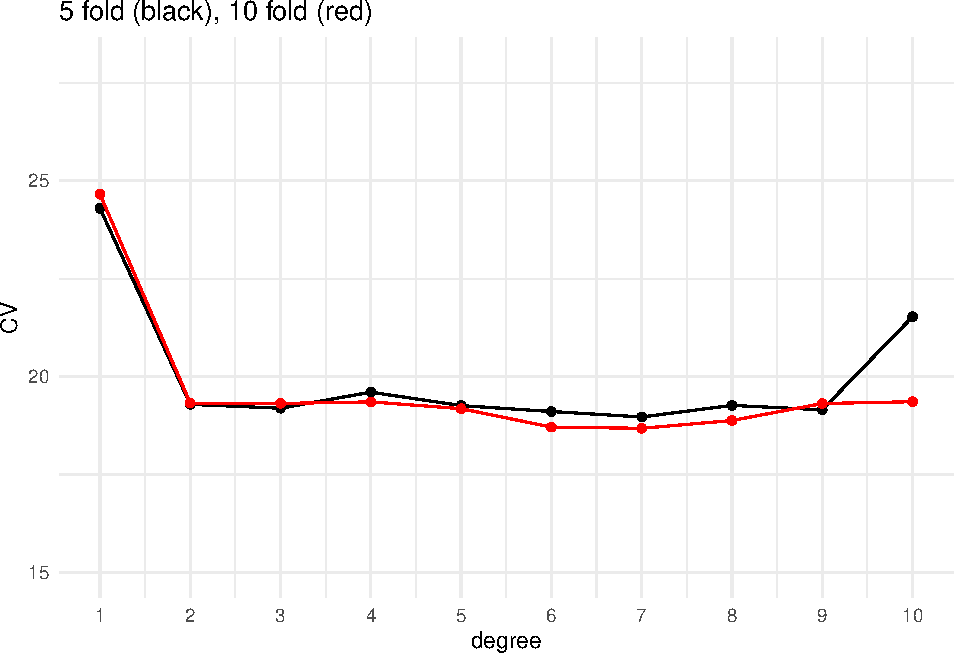
\includegraphics{5Resample_files/figure-latex/unnamed-chunk-5-1.pdf}

\begin{center}\rule{0.5\linewidth}{\linethickness}\end{center}

\tiny

\begin{Shaded}
\begin{Highlighting}[]
\KeywordTok{library}\NormalTok{(ISLR)}
\KeywordTok{library}\NormalTok{(boot)}
\KeywordTok{library}\NormalTok{(ggplot2)}
\KeywordTok{set.seed}\NormalTok{(}\DecValTok{123}\NormalTok{)}
\NormalTok{n =}\StringTok{ }\KeywordTok{dim}\NormalTok{(Auto)[}\DecValTok{1}\NormalTok{]}
\NormalTok{testMSEvec5 =}\StringTok{ }\OtherTok{NULL}
\NormalTok{testMSEvec10 =}\StringTok{ }\OtherTok{NULL}
\NormalTok{start =}\StringTok{ }\KeywordTok{Sys.time}\NormalTok{()}
\ControlFlowTok{for}\NormalTok{ (polydeg }\ControlFlowTok{in} \DecValTok{1}\OperatorTok{:}\DecValTok{10}\NormalTok{) \{}
\NormalTok{    glm.fit =}\StringTok{ }\KeywordTok{glm}\NormalTok{(mpg }\OperatorTok{~}\StringTok{ }\KeywordTok{poly}\NormalTok{(horsepower, polydeg), }\DataTypeTok{data =}\NormalTok{ Auto)}
\NormalTok{    glm.cv5 =}\StringTok{ }\KeywordTok{cv.glm}\NormalTok{(Auto, glm.fit, }\DataTypeTok{K =} \DecValTok{5}\NormalTok{)}
\NormalTok{    glm.cv10 =}\StringTok{ }\KeywordTok{cv.glm}\NormalTok{(Auto, glm.fit, }\DataTypeTok{K =} \DecValTok{10}\NormalTok{)}
\NormalTok{    testMSEvec5 =}\StringTok{ }\KeywordTok{c}\NormalTok{(testMSEvec5, glm.cv5}\OperatorTok{$}\NormalTok{delta[}\DecValTok{1}\NormalTok{])}
\NormalTok{    testMSEvec10 =}\StringTok{ }\KeywordTok{c}\NormalTok{(testMSEvec10, glm.cv10}\OperatorTok{$}\NormalTok{delta[}\DecValTok{1}\NormalTok{])}
\NormalTok{\}}
\NormalTok{stopp =}\StringTok{ }\KeywordTok{Sys.time}\NormalTok{()}
\NormalTok{yrange =}\StringTok{ }\KeywordTok{c}\NormalTok{(}\DecValTok{15}\NormalTok{, }\DecValTok{28}\NormalTok{)}
\NormalTok{plotdf =}\StringTok{ }\KeywordTok{data.frame}\NormalTok{(}\DataTypeTok{testMSE5 =}\NormalTok{ testMSEvec5, }\DataTypeTok{degree =} \DecValTok{1}\OperatorTok{:}\DecValTok{10}\NormalTok{)}
\NormalTok{g0 =}\StringTok{ }\KeywordTok{ggplot}\NormalTok{(plotdf, }\KeywordTok{aes}\NormalTok{(}\DataTypeTok{x =}\NormalTok{ degree, }\DataTypeTok{y =}\NormalTok{ testMSE5)) }\OperatorTok{+}\StringTok{ }\KeywordTok{geom_line}\NormalTok{() }\OperatorTok{+}\StringTok{ }\KeywordTok{geom_point}\NormalTok{() }\OperatorTok{+}\StringTok{ }
\StringTok{    }\KeywordTok{scale_y_continuous}\NormalTok{(}\DataTypeTok{limits =}\NormalTok{ yrange) }\OperatorTok{+}\StringTok{ }\KeywordTok{scale_x_continuous}\NormalTok{(}\DataTypeTok{breaks =} \DecValTok{1}\OperatorTok{:}\DecValTok{10}\NormalTok{) }\OperatorTok{+}\StringTok{ }
\StringTok{    }\KeywordTok{labs}\NormalTok{(}\DataTypeTok{y =} \StringTok{"CV"}\NormalTok{) }\OperatorTok{+}\StringTok{ }\KeywordTok{ggtitle}\NormalTok{(}\StringTok{"5 and 10 fold CV"}\NormalTok{)}
\NormalTok{g0 }\OperatorTok{+}\StringTok{ }\KeywordTok{geom_line}\NormalTok{(}\KeywordTok{aes}\NormalTok{(}\DataTypeTok{y =}\NormalTok{ testMSEvec10), }\DataTypeTok{colour =} \StringTok{"red"}\NormalTok{) }\OperatorTok{+}\StringTok{ }\KeywordTok{geom_point}\NormalTok{(}\KeywordTok{aes}\NormalTok{(}\DataTypeTok{y =}\NormalTok{ testMSEvec10), }
    \DataTypeTok{colour =} \StringTok{"red"}\NormalTok{) }\OperatorTok{+}\StringTok{ }\KeywordTok{ggtitle}\NormalTok{(}\StringTok{"5 fold (black), 10 fold (red)"}\NormalTok{) }\OperatorTok{+}\StringTok{ }\KeywordTok{theme_minimal}\NormalTok{()}
\end{Highlighting}
\end{Shaded}

\normalsize

\begin{center}\rule{0.5\linewidth}{\linethickness}\end{center}

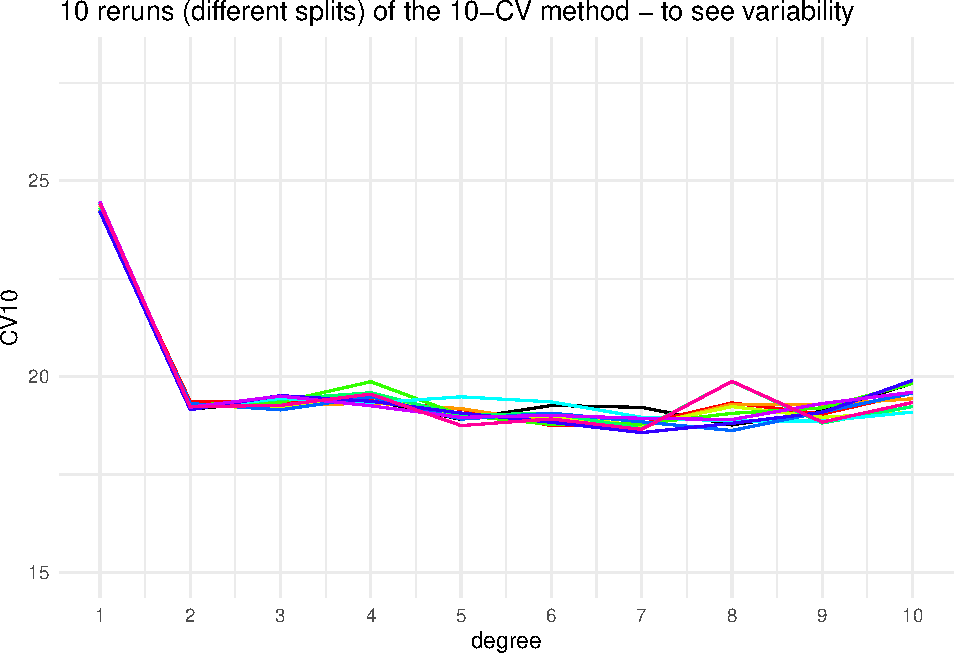
\includegraphics{5Resample_files/figure-latex/unnamed-chunk-7-1.pdf}

\begin{center}\rule{0.5\linewidth}{\linethickness}\end{center}

\hypertarget{issues-with-k-fold-cross-validation}{%
\subsubsection{\texorpdfstring{Issues with \(k\)-fold
cross-validation}{Issues with k-fold cross-validation}}\label{issues-with-k-fold-cross-validation}}

\begin{enumerate}
\def\labelenumi{\arabic{enumi}.}
\tightlist
\item
  As for the validation set, the result may vary according to how the
  folds are made, but the variation is in general lower than for the
  validation set approach.
\item
  Computational issues: less work with \(k=5\) or 10 than LOOCV.
\item
  The training set is \((k-1)/k\) of the original data set - this will
  give and estimate of the prediction error that is biased upwards.
\item
  This bias is the smalles when \(k=n\) (LOOCV), but we know that LOOCV
  has high variance.
\item
  This is way often \(k=5\) or \(k=10\) is used as a compromise between
  3 and 4.
\end{enumerate}

\begin{center}\rule{0.5\linewidth}{\linethickness}\end{center}

\hypertarget{choosing-the-best-model}{%
\subsubsection{Choosing the best model}\label{choosing-the-best-model}}

Remember that we \emph{randomly divide} the data into \(k\) folds and
then perform the CV for all possible model that we want to choose
between.

We have not directly indicated that there is a model parameter (maybe
\(K\) in KNN), say \(\theta\), involved to calculate \(\text{CV}_j\),
\(j=1,\ldots, k\)

\textbf{Smallest CV-error:}

\begin{itemize}
\tightlist
\item
  Based on the CV-plot we may choose the best model (\(\theta\)) to be
  the model with the smallest \({\text{CV}_k}\).
\item
  We then fit this model using the whole data set (not the test part,
  that is still kept away), and evaluate the performance on the test
  set.
\end{itemize}

\begin{center}\rule{0.5\linewidth}{\linethickness}\end{center}

\textbf{One standard error rule:}

Denote by \(\text{MSE}_j(\theta)\), \(j=1,\ldots, k\) the \(k\) parts of
the MSE that together give the \(\text{CV}_k\).

We can compute the sample standard deviation of
\(\text{MSE}_j(\theta)\), \(j=1,\ldots, k\) for each value of the
complexity parameter \(\theta\), say \(\text{SD} (\theta)\) and then use
\(\text{SE}(\theta)=\text{SD}(\theta)/\sqrt{k}\) as the standard
deviation of \(\text{CV}_k\).

The \emph{one standard error rule} is to choose the simplest
(e.g.~highest value of K in KNN or lowest polynomial degree in the
polynomial example) \(\theta\), that is, we move \(\theta\) in the
direction of simplicity until it ceases to be true that

\[\text{CV}(\theta)\le \text{CV}(\hat{\theta})+ \text{SE}(\hat{\theta})\]

This will be the simplest model whose error is within one standard error
of the minimal error.

\begin{center}\rule{0.5\linewidth}{\linethickness}\end{center}

\hypertarget{k-fold-cross-validation-in-classification}{%
\subsubsection{\texorpdfstring{\(k\)-fold cross-validation in
classification}{k-fold cross-validation in classification}}\label{k-fold-cross-validation-in-classification}}

\begin{itemize}
\tightlist
\item
  what do we need to change from our regression set-up?
\end{itemize}

For LOOCV \(\hat{y}_i\) is the fit for observation \(i\) obtained from
the data with observations \(i\) removed, and
\({\text{Err}_i}=I(y_i\neq \hat{y}_i)\) . LOOCV is then

\[CV_{n}=\frac{1}{n} \sum_{i=1}^n {\text{Err}_i}\]

The \(k\)-fold CV is defined analogously.

\begin{center}\rule{0.5\linewidth}{\linethickness}\end{center}

\hypertarget{exam-2018-problem-1-k-nearest-neighbour-regression}{%
\subsubsection{\texorpdfstring{Exam 2018, Problem 1: \(K\)-nearest
neighbour
regression}{Exam 2018, Problem 1: K-nearest neighbour regression}}\label{exam-2018-problem-1-k-nearest-neighbour-regression}}

\textbf{Q1:} Write down the formula for the \(K\)-nearest neighbour
regression curve estimate at a covariate value \(x_0\), and explain your
notation.

\[\hat{f}(x_0)=\frac{1}{K}\sum_{i\in \mathcal{N}_0} y_i\]

Given an integer \(K\) and a test observation \(x_0\), the KNN
regression first identifies the \(K\) points in the training data that
are closest (Euclidean distance) to \(x_0\), represented by
\(\mathcal{N}_0\). It then estimates the regression curve at \(x_0\) as
the average of the response values for the training observations in
\(\mathcal{N}_0\).

Common mistakes in the exam papers: many answered how to do
KNN-classification. In addition some wrote either \(x_i\) or \(f(x_i)\)
in place of \(y_i\) in the formula above.

\begin{center}\rule{0.5\linewidth}{\linethickness}\end{center}

\textbf{Q3:} Explain how 5-fold is performed, and specify which error
measure you would use. Your answer should include a formula to specify
how the validation error is calculated. A drawing would also be
appreciated.

We look at a set of possible values for \(K\) in the KNN, for example
\(K=(1,2,3,5,7,9,15,25,50,100)\). First we devide the data into a
training set and a test set - and lock away the test set for model
evaluation.

We work now with the training set.

\begin{center}\rule{0.5\linewidth}{\linethickness}\end{center}

\textbf{5-fold CV:} we divide the training data randomly into 5 folds of
size \(n/5\) each and call the folds \(j=1\), to \(j=5\).

For each value of \(K\) we do the following.

For \(j=1,\ldots,5\):

\begin{itemize}
\tightlist
\item
  use the \(4n/5\) observations from the folds except fold \(j\) to
  define the \(K\)-neighbourhood \(\mathcal{N}_0\) for each of the
  observations in the \(j\)th fold
\item
  the observations in the \(j\)th fold is left out and is the validation
  set, there are \(n/5\) observations - and we denote them
  \((x_{0jl},y_{0jl})\),
\item
  we then estimate
  \(\hat{f}(x_{0jl})=\frac{1}{K}\sum_{i\in \mathcal{N}_0} y_i\).
\item
  We calculate the error in the \(j\)th fold of the validation set as
  \(\sum_{l} (y_{0jl}-\hat{f}(x_{0jl}))^2\) where the \(j\) is for the
  validation fold
\end{itemize}

The total error on the validation set is thus the validation
MSE=\(\frac{1}{n}\sum_{j=1}^5 \sum_{l}(y_{0jl}-\hat{f}(x_{0jl}))^2\).

So, for each value of \(K\) we get an estimate of the validation MSE.
Finally, we choose the value of \(K\) that gives the lowest validation
MSE.

Common mistakes: many forget to shuffle data. Some forget to explain how
this is related to choosing the number of neighbours in KNN (only focus
on the 5-fold CV process) - that is, relate this to the setting of the
problem. A few mention the error measure for classification.

\begin{center}\rule{0.5\linewidth}{\linethickness}\end{center}

\textbf{Q4:} In your opinion, would you prefer the leave-one-out
cross-validation or the 5-fold cross-validation method? Justify your
answer.

The LOOCV would give a less biased estimate of the MSE on a test set,
since the sample size used \((n-1)\) is close to the sample size to be
used in the real world situation \((n)\), but the LOOCV will be variable
(the variance of the validation MSE is high).

On the other hand the 5-fold CV would give a biased estimate of the MSE
on a test set since the sample size used is 4/5 of the sample size that
would be used in the real world situation. However, the variance will be
lower than for the LOOCV.

When it comes to computational complexity we have in general that with
LOOCV we need to fit \(n\) models but with 5-fold only 5. However, for
KNN-regression there is really no model fitting, we only choose the
\(K\) closest neighbours in the training part of the data. This means
that LOOCV should not be more time consuming than 5-fold for KNN.

There is no ``true'' answer here -- and arguments for both solutions can
be given.

Common mistakes: many did not talk about bias, variance and
computational complexity, a few made mistakes on the comparison of LOOCV
and 5-fold CV with respect to bias and variance.

\begin{center}\rule{0.5\linewidth}{\linethickness}\end{center}

\hypertarget{can-we-use-cv-for-model-assessment}{%
\subsubsection{Can we use CV for model
assessment?}\label{can-we-use-cv-for-model-assessment}}

Assume that we have a method where we not need to perform model
selection (maybe this is done using the methods from Module 6, that is
AIC or lasso), but want to perform model assessment based on all our
data.

Then we can use CV with all data (then the validation part is really the
test part) and report on the model performance using the validation
parts of the data as above.

\hypertarget{can-we-use-cv-both-for-model-selection-and-model-assessment}{%
\subsubsection{Can we use CV both for model selection and model
assessment?}\label{can-we-use-cv-both-for-model-selection-and-model-assessment}}

Then you can use two layers of CV - also called \emph{nested CV}. See
drawing in class.

\begin{center}\rule{0.5\linewidth}{\linethickness}\end{center}

\hypertarget{the-right-and-the-wrong-way-to-do-cross-validation}{%
\subsection{The right and the wrong way to do
cross-validation}\label{the-right-and-the-wrong-way-to-do-cross-validation}}

\href{https://lagunita.stanford.edu/c4x/HumanitiesScience/StatLearning/asset/cv_boot.pdf}{ISL
book slides, page 17}: model assessment.

\begin{itemize}
\tightlist
\item
  We have a two-class problem and would like to use a simple
  classification method, however,
\item
  we have many possible predictors \(p=5000\) and not so big sample size
  \(n=50\).
\end{itemize}

We use this strategy to produce a classifier:

\begin{enumerate}
\def\labelenumi{\arabic{enumi}.}
\tightlist
\item
  We calculate the correlation between the class label and each of the
  \(p\) predictors, and choose the \(d=25\) predictors that have the
  highest (absolute value) correlation with the class label. (We need to
  have \(d<n\) to fit the logistic regression uniquely.)
\item
  Then we fit our classifier (here: logistic regression) using only the
  \(d=25\) predictors.
\end{enumerate}

How can we use cross-validation to produce an estimate of the
performance of this classifier?

\textbf{Q}: Can we apply cross-validation only to step 2? Why or why
not?

\begin{center}\rule{0.5\linewidth}{\linethickness}\end{center}

Can we apply cross-validation only to step 2?

\textbf{A:} No, step 1 is part of the training procedure (the class
labels are used) and must be part of the CV to give an honest estimate
of the performance of the classifier.

\begin{itemize}
\tightlist
\item
  Wrong: Apply cross-validation in step 2.
\item
  Right: Apply cross-validation to steps 1 and 2.
\end{itemize}

We will see in the Recommended Exercises that doing the wrong thing can
give a misclassification error approximately 0 - even if the ``true''
rate is 50\%.

\begin{center}\rule{0.5\linewidth}{\linethickness}\end{center}

\hypertarget{selection-bias-in-gene-extraction-on-the-basis-of-microarray-gene-expression-data}{%
\subsubsection{Selection bias in gene extraction on the basis of
microarray gene-expression
data}\label{selection-bias-in-gene-extraction-on-the-basis-of-microarray-gene-expression-data}}

Article by \href{http://www.pnas.org/content/99/10/6562}{Christophe
Ambroise and Geoffrey J. McLachlan, PNAS 2002}: Direct quotation from
the abstract of the article follows.

\begin{itemize}
\tightlist
\item
  In the context of cancer diagnosis and treatment, we consider the
  problem of constructing an accurate prediction rule on the basis of a
  relatively small number of tumor tissue samples of known type
  containing the expression data on very many (possibly thousands)
  genes.
\item
  Recently, results have been presented in the literature suggesting
  that it is possible to construct a prediction rule from only a few
  genes such that it has a negligible prediction error rate.
\item
  However, in these results the test error or the leave-one-out
  cross-validated error is calculated without allowance for the
  selection bias.
\end{itemize}

\begin{center}\rule{0.5\linewidth}{\linethickness}\end{center}

\begin{itemize}
\tightlist
\item
  There is no allowance because the rule is either tested on tissue
  samples that were used in the first instance to select the genes being
  used in the rule or because the cross-validation of the rule is not
  external to the selection process; that is, gene selection is not
  performed in training the rule at each stage of the crossvalidation
  process.
\item
  We describe how in practice the selection bias can be assessed and
  corrected for by either performing a crossvalidation or applying the
  bootstrap external to the selection process.
\item
  We recommend using 10-fold rather than leave-one-out cross-validation,
  and concerning the bootstrap, we suggest using the so-called .632
  bootstrap error estimate designed to handle overfitted prediction
  rules.
\item
  Using two published data sets, we demonstrate that when correction is
  made for the selection bias, the cross-validated error is no longer
  zero for a subset of only a few genes.
\end{itemize}

\begin{center}\rule{0.5\linewidth}{\linethickness}\end{center}

\hypertarget{recommended-exercises-on-cross-validation}{%
\section{Recommended exercises on
cross-validation}\label{recommended-exercises-on-cross-validation}}

\hypertarget{problem-1-explain-how-k-fold-cross-validation-is-implemented}{%
\subsection{\texorpdfstring{Problem 1: Explain how \(k\)-fold
cross-validation is
implemented}{Problem 1: Explain how k-fold cross-validation is implemented}}\label{problem-1-explain-how-k-fold-cross-validation-is-implemented}}

\begin{itemize}
\tightlist
\item
  draw a figure,
\item
  specify algorithmically what is done,
\item
  and in particular how the ``results'' from each fold are aggregated,
\item
  relate to one example from regression (maybe is complexity wrt
  polynomials of increasing degree in multiple linear regression or
  \(K\) in KNN-regression?)
\item
  relate to one example from classification (maybe is complexity wrt
  polynomials of increasing degree in logistic regression or \(K\) in
  KNN-classification?)
\end{itemize}

Hint: the words ``loss function'', ``fold'', ``training'',
``validation'' are central.

\begin{center}\rule{0.5\linewidth}{\linethickness}\end{center}

\hypertarget{problem-2-what-are-the-advantages-and-disadvantages-of-k-fold-cross-validation}{%
\subsection{\texorpdfstring{Problem 2: What are the advantages and
disadvantages of \(k\)-fold
cross-validation}{Problem 2: What are the advantages and disadvantages of k-fold cross-validation}}\label{problem-2-what-are-the-advantages-and-disadvantages-of-k-fold-cross-validation}}

relative to

\begin{itemize}
\tightlist
\item
  the validation set approach
\item
  leave one out cross-validation (LOOCV)
\item
  what are recommended values for \(k\), and why?
\end{itemize}

Hint: the words ``bias'', ``variance'' and ``computational complexity''
should be included.

\begin{center}\rule{0.5\linewidth}{\linethickness}\end{center}

\hypertarget{problem-3-selection-bias-and-the-wrong-way-to-do-cv.}{%
\subsection{Problem 3: Selection bias and the ``wrong way to do
CV''.}\label{problem-3-selection-bias-and-the-wrong-way-to-do-cv.}}

The task here is to devise an algorithm to ``prove'' that the wrong way
is wrong and that the right way is right.

\begin{enumerate}
\def\labelenumi{\alph{enumi}.}
\tightlist
\item
  What are the steps of such an algorithm? Write down a suggestion.
  Hint: how do you generate data for predictors and class labels, how do
  you do the classification task, where is the CV in the correct way and
  wrong way inserted into your algorithm? Can you make a schematic
  drawing of the right and the wrong way? Hint:
  \href{https://lagunita.stanford.edu/c4x/HumanitiesScience/StatLearning/asset/cv_boot.pdf}{ISL
  book slides, page 20+21} - but you can do better?
\end{enumerate}

\begin{center}\rule{0.5\linewidth}{\linethickness}\end{center}

\begin{enumerate}
\def\labelenumi{\alph{enumi}.}
\setcounter{enumi}{1}
\tightlist
\item
  One possible version of this is presented in the R-code below. Go
  through the code and explain what is done in each step, then run the
  code and observe if the results are in agreement with what you
  expected. Make changes to the R-code if you want to test out different
  strategies.
\end{enumerate}

\begin{Shaded}
\begin{Highlighting}[]
\KeywordTok{library}\NormalTok{(boot)}
\CommentTok{# GENERATE DATA reproducible}
\KeywordTok{set.seed}\NormalTok{(}\DecValTok{4268}\NormalTok{)}
\NormalTok{n =}\StringTok{ }\DecValTok{50}  \CommentTok{#number of observations}
\NormalTok{p =}\StringTok{ }\DecValTok{5000}  \CommentTok{#number of predictors}
\NormalTok{d =}\StringTok{ }\DecValTok{25}  \CommentTok{#top correlated predictors chosen}
\NormalTok{kfold =}\StringTok{ }\DecValTok{10}
\CommentTok{# generating predictor data}
\NormalTok{xs =}\StringTok{ }\KeywordTok{matrix}\NormalTok{(}\KeywordTok{rnorm}\NormalTok{(n }\OperatorTok{*}\StringTok{ }\NormalTok{p, }\DecValTok{0}\NormalTok{, }\DecValTok{4}\NormalTok{), }\DataTypeTok{ncol =}\NormalTok{ p, }\DataTypeTok{nrow =}\NormalTok{ n)  }\CommentTok{#simple way to to uncorrelated predictors}
\KeywordTok{dim}\NormalTok{(xs)  }\CommentTok{# n times p}
\CommentTok{# generate class labels independent of predictors - so if all}
\CommentTok{# classifies as class 1 we expect 50% errors in general}
\NormalTok{ys =}\StringTok{ }\KeywordTok{c}\NormalTok{(}\KeywordTok{rep}\NormalTok{(}\DecValTok{0}\NormalTok{, n}\OperatorTok{/}\DecValTok{2}\NormalTok{), }\KeywordTok{rep}\NormalTok{(}\DecValTok{1}\NormalTok{, n}\OperatorTok{/}\DecValTok{2}\NormalTok{))  }\CommentTok{#now really 50% of each}
\KeywordTok{table}\NormalTok{(ys)}

\CommentTok{# WRONG CV - using cv.glm here select the most correlated predictors}
\CommentTok{# outside the CV}
\NormalTok{corrs =}\StringTok{ }\KeywordTok{apply}\NormalTok{(xs, }\DecValTok{2}\NormalTok{, cor, }\DataTypeTok{y =}\NormalTok{ ys)}
\KeywordTok{hist}\NormalTok{(corrs)}
\NormalTok{selected =}\StringTok{ }\KeywordTok{order}\NormalTok{(corrs}\OperatorTok{^}\DecValTok{2}\NormalTok{, }\DataTypeTok{decreasing =} \OtherTok{TRUE}\NormalTok{)[}\DecValTok{1}\OperatorTok{:}\NormalTok{d]  }\CommentTok{#top d correlated selected}
\NormalTok{data =}\StringTok{ }\KeywordTok{data.frame}\NormalTok{(ys, xs[, selected])}
\CommentTok{# apply(xs[,selected],2,cor,y=ys) yes, ave the most correlated then}
\CommentTok{# cv around the fitting of the classifier - use logistic regression}
\CommentTok{# and built in cv.glm function}
\NormalTok{logfit =}\StringTok{ }\KeywordTok{glm}\NormalTok{(ys }\OperatorTok{~}\StringTok{ }\NormalTok{., }\DataTypeTok{family =} \StringTok{"binomial"}\NormalTok{, }\DataTypeTok{data =}\NormalTok{ data)}
\NormalTok{cost <-}\StringTok{ }\ControlFlowTok{function}\NormalTok{(r, }\DataTypeTok{pi =} \DecValTok{0}\NormalTok{) }\KeywordTok{mean}\NormalTok{(}\KeywordTok{abs}\NormalTok{(r }\OperatorTok{-}\StringTok{ }\NormalTok{pi) }\OperatorTok{>}\StringTok{ }\FloatTok{0.5}\NormalTok{)}
\NormalTok{cvres =}\StringTok{ }\KeywordTok{cv.glm}\NormalTok{(}\DataTypeTok{data =}\NormalTok{ data, }\DataTypeTok{cost =}\NormalTok{ cost, }\DataTypeTok{glmfit =}\NormalTok{ logfit, }\DataTypeTok{K =}\NormalTok{ kfold)}
\NormalTok{cvres}\OperatorTok{$}\NormalTok{delta}
\CommentTok{# observe - near 0 misclassification rate}

\CommentTok{# WRONG without using cv.glm - should be similar (just added to see}
\CommentTok{# the similarity to the RIGHT version)}
\NormalTok{reorder =}\StringTok{ }\KeywordTok{sample}\NormalTok{(}\DecValTok{1}\OperatorTok{:}\NormalTok{n, }\DataTypeTok{replace =} \OtherTok{FALSE}\NormalTok{)}
\NormalTok{validclass =}\StringTok{ }\OtherTok{NULL}
\ControlFlowTok{for}\NormalTok{ (i }\ControlFlowTok{in} \DecValTok{1}\OperatorTok{:}\NormalTok{kfold) \{}
\NormalTok{    neach =}\StringTok{ }\NormalTok{n}\OperatorTok{/}\NormalTok{kfold}
\NormalTok{    trainids =}\StringTok{ }\KeywordTok{setdiff}\NormalTok{(}\DecValTok{1}\OperatorTok{:}\NormalTok{n, (((i }\OperatorTok{-}\StringTok{ }\DecValTok{1}\NormalTok{) }\OperatorTok{*}\StringTok{ }\NormalTok{neach }\OperatorTok{+}\StringTok{ }\DecValTok{1}\NormalTok{)}\OperatorTok{:}\NormalTok{(i }\OperatorTok{*}\StringTok{ }\NormalTok{neach)))}
\NormalTok{    traindata =}\StringTok{ }\KeywordTok{data.frame}\NormalTok{(xs[reorder[trainids], ], ys[reorder[trainids]])}
\NormalTok{    validdata =}\StringTok{ }\KeywordTok{data.frame}\NormalTok{(xs[reorder[}\OperatorTok{-}\NormalTok{trainids], ], ys[reorder[}\OperatorTok{-}\NormalTok{trainids]])}
    \KeywordTok{colnames}\NormalTok{(traindata) =}\StringTok{ }\KeywordTok{colnames}\NormalTok{(validdata) =}\StringTok{ }\KeywordTok{c}\NormalTok{(}\KeywordTok{paste}\NormalTok{(}\StringTok{"X"}\NormalTok{, }\DecValTok{1}\OperatorTok{:}\NormalTok{p), }\StringTok{"y"}\NormalTok{)}
\NormalTok{    data =}\StringTok{ }\NormalTok{traindata[, }\KeywordTok{c}\NormalTok{(selected, p }\OperatorTok{+}\StringTok{ }\DecValTok{1}\NormalTok{)]}
\NormalTok{    trainlogfit =}\StringTok{ }\KeywordTok{glm}\NormalTok{(y }\OperatorTok{~}\StringTok{ }\NormalTok{., }\DataTypeTok{family =} \StringTok{"binomial"}\NormalTok{, }\DataTypeTok{data =}\NormalTok{ data)}
\NormalTok{    pred =}\StringTok{ }\KeywordTok{plogis}\NormalTok{(}\KeywordTok{predict.glm}\NormalTok{(trainlogfit, }\DataTypeTok{newdata =}\NormalTok{ validdata[, selected]))}
    \KeywordTok{print}\NormalTok{(pred)}
\NormalTok{    validclass =}\StringTok{ }\KeywordTok{c}\NormalTok{(validclass, }\KeywordTok{ifelse}\NormalTok{(pred }\OperatorTok{>}\StringTok{ }\FloatTok{0.5}\NormalTok{, }\DecValTok{1}\NormalTok{, }\DecValTok{0}\NormalTok{))}
\NormalTok{\}}
\KeywordTok{table}\NormalTok{(ys[reorder], validclass)}
\DecValTok{1} \OperatorTok{-}\StringTok{ }\KeywordTok{sum}\NormalTok{(}\KeywordTok{diag}\NormalTok{(}\KeywordTok{table}\NormalTok{(ys[reorder], validclass)))}\OperatorTok{/}\NormalTok{n}

\CommentTok{# CORRECT CV}
\NormalTok{reorder =}\StringTok{ }\KeywordTok{sample}\NormalTok{(}\DecValTok{1}\OperatorTok{:}\NormalTok{n, }\DataTypeTok{replace =} \OtherTok{FALSE}\NormalTok{)}
\NormalTok{validclass =}\StringTok{ }\OtherTok{NULL}
\ControlFlowTok{for}\NormalTok{ (i }\ControlFlowTok{in} \DecValTok{1}\OperatorTok{:}\NormalTok{kfold) \{}
\NormalTok{    neach =}\StringTok{ }\NormalTok{n}\OperatorTok{/}\NormalTok{kfold}
\NormalTok{    trainids =}\StringTok{ }\KeywordTok{setdiff}\NormalTok{(}\DecValTok{1}\OperatorTok{:}\NormalTok{n, (((i }\OperatorTok{-}\StringTok{ }\DecValTok{1}\NormalTok{) }\OperatorTok{*}\StringTok{ }\NormalTok{neach }\OperatorTok{+}\StringTok{ }\DecValTok{1}\NormalTok{)}\OperatorTok{:}\NormalTok{(i }\OperatorTok{*}\StringTok{ }\NormalTok{neach)))}
\NormalTok{    traindata =}\StringTok{ }\KeywordTok{data.frame}\NormalTok{(xs[reorder[trainids], ], ys[reorder[trainids]])}
\NormalTok{    validdata =}\StringTok{ }\KeywordTok{data.frame}\NormalTok{(xs[reorder[}\OperatorTok{-}\NormalTok{trainids], ], ys[reorder[}\OperatorTok{-}\NormalTok{trainids]])}
    \KeywordTok{colnames}\NormalTok{(traindata) =}\StringTok{ }\KeywordTok{colnames}\NormalTok{(validdata) =}\StringTok{ }\KeywordTok{c}\NormalTok{(}\KeywordTok{paste}\NormalTok{(}\StringTok{"X"}\NormalTok{, }\DecValTok{1}\OperatorTok{:}\NormalTok{p), }\StringTok{"y"}\NormalTok{)}
\NormalTok{    foldcorrs =}\StringTok{ }\KeywordTok{apply}\NormalTok{(traindata[, }\DecValTok{1}\OperatorTok{:}\NormalTok{p], }\DecValTok{2}\NormalTok{, cor, }\DataTypeTok{y =}\NormalTok{ traindata[, p }\OperatorTok{+}\StringTok{ }\DecValTok{1}\NormalTok{])}
\NormalTok{    selected =}\StringTok{ }\KeywordTok{order}\NormalTok{(foldcorrs}\OperatorTok{^}\DecValTok{2}\NormalTok{, }\DataTypeTok{decreasing =} \OtherTok{TRUE}\NormalTok{)[}\DecValTok{1}\OperatorTok{:}\NormalTok{d]  }\CommentTok{#top d correlated selected}
\NormalTok{    data =}\StringTok{ }\NormalTok{traindata[, }\KeywordTok{c}\NormalTok{(selected, p }\OperatorTok{+}\StringTok{ }\DecValTok{1}\NormalTok{)]}
\NormalTok{    trainlogfit =}\StringTok{ }\KeywordTok{glm}\NormalTok{(y }\OperatorTok{~}\StringTok{ }\NormalTok{., }\DataTypeTok{family =} \StringTok{"binomial"}\NormalTok{, }\DataTypeTok{data =}\NormalTok{ data)}
\NormalTok{    pred =}\StringTok{ }\KeywordTok{plogis}\NormalTok{(}\KeywordTok{predict.glm}\NormalTok{(trainlogfit, }\DataTypeTok{newdata =}\NormalTok{ validdata[, selected]))}
\NormalTok{    validclass =}\StringTok{ }\KeywordTok{c}\NormalTok{(validclass, }\KeywordTok{ifelse}\NormalTok{(pred }\OperatorTok{>}\StringTok{ }\FloatTok{0.5}\NormalTok{, }\DecValTok{1}\NormalTok{, }\DecValTok{0}\NormalTok{))}
\NormalTok{\}}
\KeywordTok{table}\NormalTok{(ys[reorder], validclass)}
\DecValTok{1} \OperatorTok{-}\StringTok{ }\KeywordTok{sum}\NormalTok{(}\KeywordTok{diag}\NormalTok{(}\KeywordTok{table}\NormalTok{(ys[reorder], validclass)))}\OperatorTok{/}\NormalTok{n}
\end{Highlighting}
\end{Shaded}

\begin{center}\rule{0.5\linewidth}{\linethickness}\end{center}

\hypertarget{the-bootstrap}{%
\section{The Bootstrap}\label{the-bootstrap}}

\begin{itemize}
\tightlist
\item
  flexible and powerful statistical tool that can be used to quantify
  \emph{uncertainty} associated with an estimator or statistical
  learning method
\item
  we will look at getting an estimate for the standard error of a sample
  median and of a regression coefficient
\item
  in Module 8 - bootstrapping is the core of the \emph{ensemble method}
  referred to at \emph{bagging}=bootstrap aggregation,
\item
  in TMA4300 Computation statistics - a lot more theory on the
  bootstrap.
\end{itemize}

\begin{center}\rule{0.5\linewidth}{\linethickness}\end{center}

The inventor: Bradley Efron in 1979 -
\href{https://www.youtube.com/watch?v=6l9V1sINzhE}{see interview}.

The name? \emph{To pull oneself up by one's bootstraps} from ``The
Surprising Adventures of Baron Munchausen'' by Rudolph Erich Raspe:

\emph{The Baron had fallen to the bottom of a deep lake. Just when it
looked like all was lost, he thought to pick himself up by his own
bootstraps.}

\textbf{Idea: Use the data itself to get more information about a
statistic (an estimator).}

\begin{center}\rule{0.5\linewidth}{\linethickness}\end{center}

\hypertarget{example-the-standard-deviation-of-the-sample-median}{%
\subsection{Example: the standard deviation of the sample
median?}\label{example-the-standard-deviation-of-the-sample-median}}

Assume that we observe a random sample \(X_1, X_2, \ldots, X_n\) from an
unknown probability distribution \(f\). We are interesting in saying
something about the population median, and to do that we calculate the
sample median \(\tilde{X}\). But, how accurate is \(\tilde{X}\) as an
estimator?

The bootstrap was introduced as a computer-based method to estimate the
standard deviation of an estimator, for example our estimator
\(\tilde{X}\).

But, before we look at the bootstrap method, first we assume that we
know \(F\) and can sample from \(F\), and use simulations to answer our
question.

\begin{center}\rule{0.5\linewidth}{\linethickness}\end{center}

\begin{Shaded}
\begin{Highlighting}[]
\KeywordTok{set.seed}\NormalTok{(}\DecValTok{123}\NormalTok{)}
\NormalTok{n =}\StringTok{ }\DecValTok{101}
\NormalTok{B =}\StringTok{ }\DecValTok{1000}
\NormalTok{estimator =}\StringTok{ }\KeywordTok{rep}\NormalTok{(}\OtherTok{NA}\NormalTok{, B)}
\ControlFlowTok{for}\NormalTok{ (b }\ControlFlowTok{in} \DecValTok{1}\OperatorTok{:}\NormalTok{B) \{}
\NormalTok{    xs =}\StringTok{ }\KeywordTok{rnorm}\NormalTok{(n)}
\NormalTok{    estimator[b] =}\StringTok{ }\KeywordTok{median}\NormalTok{(xs)}
\NormalTok{\}}
\KeywordTok{sd}\NormalTok{(estimator)}
\end{Highlighting}
\end{Shaded}

\begin{verbatim}
## [1] 0.1259035
\end{verbatim}

\begin{Shaded}
\begin{Highlighting}[]
\CommentTok{# approximation for large samples (sd of median of standard normal)}
\FloatTok{1.253} \OperatorTok{*}\StringTok{ }\DecValTok{1}\OperatorTok{/}\KeywordTok{sqrt}\NormalTok{(n)}
\end{Highlighting}
\end{Shaded}

\begin{verbatim}
## [1] 0.1246782
\end{verbatim}

\begin{center}\rule{0.5\linewidth}{\linethickness}\end{center}

\begin{Shaded}
\begin{Highlighting}[]
\KeywordTok{ggplot}\NormalTok{(}\DataTypeTok{data =} \KeywordTok{data.frame}\NormalTok{(}\DataTypeTok{x =}\NormalTok{ estimator), }\KeywordTok{aes}\NormalTok{(}\DataTypeTok{x =}\NormalTok{ x)) }\OperatorTok{+}\StringTok{ }\KeywordTok{geom_density}\NormalTok{()}
\end{Highlighting}
\end{Shaded}

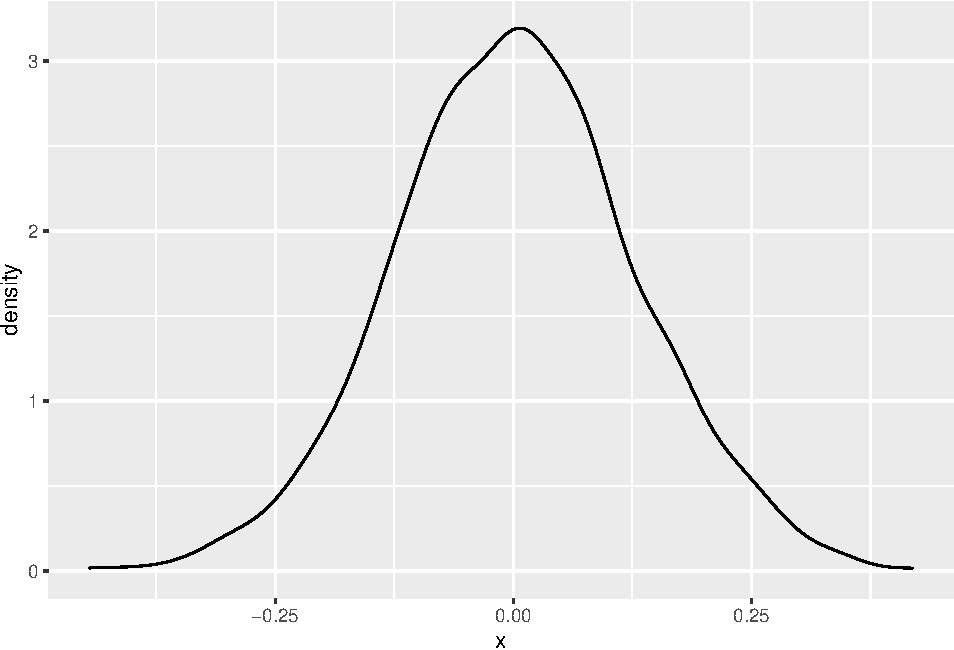
\includegraphics{5Resample_files/figure-latex/unnamed-chunk-10-1.pdf}

\begin{center}\rule{0.5\linewidth}{\linethickness}\end{center}

\hypertarget{moving-from-simulation-to-bootstrapping}{%
\subsection{Moving from simulation to
bootstrapping}\label{moving-from-simulation-to-bootstrapping}}

The bootstrap method is using the observed data to estimate the
\emph{empirical distribution} \(\hat{f}\), that is each observed value
of \(x\) is given probability \(1/n\).

A \emph{bootstrap sample} \(X^*_1,X^*_2,\ldots, X^*_n\) is a random
sample drawn from \(\hat{f}\).

A simple way to obtain the bootstrap sample is to \emph{draw with
replacement from \(X_1, X_2, \ldots, X_n\)}.

This means that our bootstrap sample consists of \(n\) members of
\(X_1, X_2, \ldots, X_n\) - some appearing 0 times, some 1, some 2, etc.

\begin{center}\rule{0.5\linewidth}{\linethickness}\end{center}

\begin{Shaded}
\begin{Highlighting}[]
\KeywordTok{set.seed}\NormalTok{(}\DecValTok{123}\NormalTok{)}
\NormalTok{n =}\StringTok{ }\DecValTok{101}
\NormalTok{original =}\StringTok{ }\KeywordTok{rnorm}\NormalTok{(n)}
\KeywordTok{median}\NormalTok{(original)}
\end{Highlighting}
\end{Shaded}

\begin{verbatim}
## [1] 0.05300423
\end{verbatim}

\begin{Shaded}
\begin{Highlighting}[]
\NormalTok{boot1 =}\StringTok{ }\KeywordTok{sample}\NormalTok{(}\DataTypeTok{x =}\NormalTok{ original, }\DataTypeTok{size =}\NormalTok{ n, }\DataTypeTok{replace =} \OtherTok{TRUE}\NormalTok{)}
\KeywordTok{table}\NormalTok{(}\KeywordTok{table}\NormalTok{(boot1))}
\end{Highlighting}
\end{Shaded}

\begin{verbatim}
## 
##  1  2  3  4 
## 34 22  5  2
\end{verbatim}

\begin{Shaded}
\begin{Highlighting}[]
\CommentTok{# how many observations have not been selected in our boot1 sample?}
\NormalTok{n }\OperatorTok{-}\StringTok{ }\KeywordTok{sum}\NormalTok{(}\KeywordTok{table}\NormalTok{(}\KeywordTok{table}\NormalTok{(boot1)))}
\end{Highlighting}
\end{Shaded}

\begin{verbatim}
## [1] 38
\end{verbatim}

\begin{Shaded}
\begin{Highlighting}[]
\KeywordTok{median}\NormalTok{(boot1)}
\end{Highlighting}
\end{Shaded}

\begin{verbatim}
## [1] -0.02854676
\end{verbatim}

\begin{center}\rule{0.5\linewidth}{\linethickness}\end{center}

\hypertarget{the-bootstrap-algorithm-for-estimating-standard-errors}{%
\subsection{The bootstrap algorithm for estimating standard
errors}\label{the-bootstrap-algorithm-for-estimating-standard-errors}}

\begin{enumerate}
\def\labelenumi{\arabic{enumi}.}
\item
  \(B\) bootstrap samples: drawn with replacement from the original data
\item
  Evaluate statistic: on each of the \(B\) bootstrap samples to get
  \(\tilde{X}^*_b\) for the \(b\)th bootstrap sample.
\item
  Estimate squared standard error by:
  \[\frac{1}{B-1}\sum_{b=1}^B (\tilde{X}^*_b-\frac{1}{B}\sum_{b=1}^B \tilde{X}^*_b)^2\]
\end{enumerate}

\begin{center}\rule{0.5\linewidth}{\linethickness}\end{center}

\hypertarget{with-for-loop-in-r}{%
\subsubsection{with for-loop in R}\label{with-for-loop-in-r}}

\begin{Shaded}
\begin{Highlighting}[]
\KeywordTok{set.seed}\NormalTok{(}\DecValTok{123}\NormalTok{)}
\NormalTok{n =}\StringTok{ }\DecValTok{101}
\NormalTok{original =}\StringTok{ }\KeywordTok{rnorm}\NormalTok{(n)}
\KeywordTok{median}\NormalTok{(original)}
\end{Highlighting}
\end{Shaded}

\begin{verbatim}
## [1] 0.05300423
\end{verbatim}

\begin{Shaded}
\begin{Highlighting}[]
\NormalTok{B =}\StringTok{ }\DecValTok{1000}
\NormalTok{estimator =}\StringTok{ }\KeywordTok{rep}\NormalTok{(}\OtherTok{NA}\NormalTok{, B)}
\ControlFlowTok{for}\NormalTok{ (b }\ControlFlowTok{in} \DecValTok{1}\OperatorTok{:}\NormalTok{B) \{}
\NormalTok{    thisboot =}\StringTok{ }\KeywordTok{sample}\NormalTok{(}\DataTypeTok{x =}\NormalTok{ original, }\DataTypeTok{size =}\NormalTok{ n, }\DataTypeTok{replace =} \OtherTok{TRUE}\NormalTok{)}
\NormalTok{    estimator[b] =}\StringTok{ }\KeywordTok{median}\NormalTok{(thisboot)}
\NormalTok{\}}
\KeywordTok{sd}\NormalTok{(estimator)}
\end{Highlighting}
\end{Shaded}

\begin{verbatim}
## [1] 0.1365448
\end{verbatim}

\begin{center}\rule{0.5\linewidth}{\linethickness}\end{center}

\begin{Shaded}
\begin{Highlighting}[]
\KeywordTok{ggplot}\NormalTok{(}\DataTypeTok{data =} \KeywordTok{data.frame}\NormalTok{(}\DataTypeTok{x =}\NormalTok{ estimator), }\KeywordTok{aes}\NormalTok{(}\DataTypeTok{x =}\NormalTok{ x)) }\OperatorTok{+}\StringTok{ }\KeywordTok{geom_density}\NormalTok{()}
\end{Highlighting}
\end{Shaded}

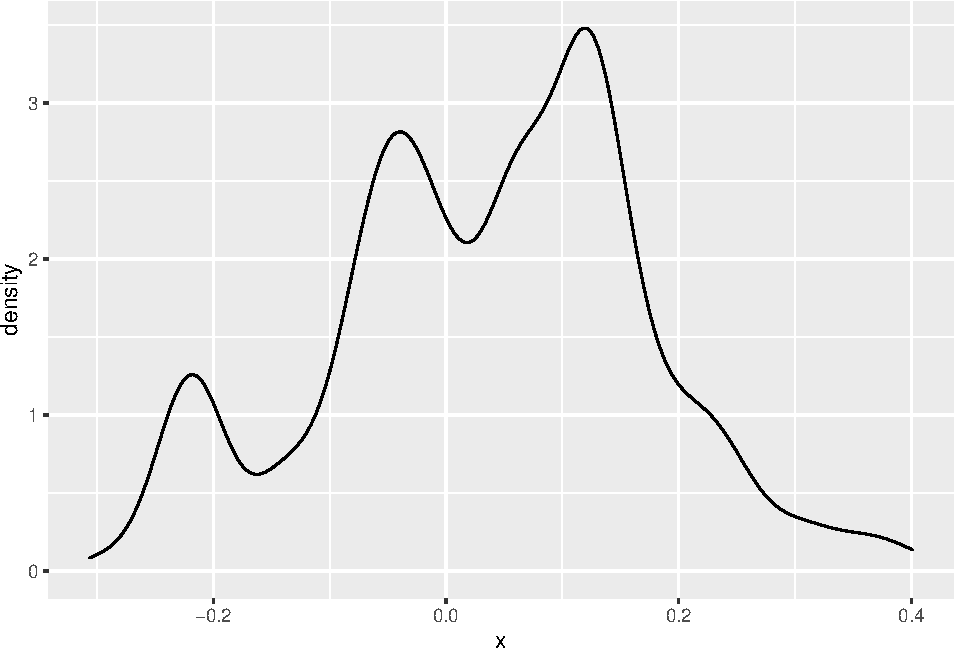
\includegraphics{5Resample_files/figure-latex/unnamed-chunk-13-1.pdf}

\begin{center}\rule{0.5\linewidth}{\linethickness}\end{center}

\hypertarget{using-built-in-boot-function-from-library-boot}{%
\subsubsection{\texorpdfstring{using built in \texttt{boot} function
from library
\texttt{boot}}{using built in boot function from library boot}}\label{using-built-in-boot-function-from-library-boot}}

\begin{Shaded}
\begin{Highlighting}[]
\KeywordTok{library}\NormalTok{(boot)}
\KeywordTok{set.seed}\NormalTok{(}\DecValTok{123}\NormalTok{)}
\NormalTok{n =}\StringTok{ }\DecValTok{101}
\NormalTok{original =}\StringTok{ }\KeywordTok{rnorm}\NormalTok{(n)}
\KeywordTok{median}\NormalTok{(original)}
\end{Highlighting}
\end{Shaded}

\begin{verbatim}
## [1] 0.05300423
\end{verbatim}

\begin{Shaded}
\begin{Highlighting}[]
\KeywordTok{summary}\NormalTok{(original)}
\end{Highlighting}
\end{Shaded}

\begin{verbatim}
##     Min.  1st Qu.   Median     Mean  3rd Qu.     Max. 
## -2.30917 -0.50232  0.05300  0.08248  0.68864  2.18733
\end{verbatim}

\begin{center}\rule{0.5\linewidth}{\linethickness}\end{center}

\begin{Shaded}
\begin{Highlighting}[]
\NormalTok{boot.median =}\StringTok{ }\ControlFlowTok{function}\NormalTok{(data, index) }\KeywordTok{return}\NormalTok{(}\KeywordTok{median}\NormalTok{(data[index]))}
\NormalTok{B =}\StringTok{ }\DecValTok{1000}
\KeywordTok{boot}\NormalTok{(original, boot.median, }\DataTypeTok{R =}\NormalTok{ B)}
\end{Highlighting}
\end{Shaded}

\begin{verbatim}
## 
## ORDINARY NONPARAMETRIC BOOTSTRAP
## 
## 
## Call:
## boot(data = original, statistic = boot.median, R = B)
## 
## 
## Bootstrap Statistics :
##       original      bias    std. error
## t1* 0.05300423 -0.01577692   0.1290482
\end{verbatim}

\begin{center}\rule{0.5\linewidth}{\linethickness}\end{center}

\hypertarget{with-or-without-replacement}{%
\subsection{With or without
replacement?}\label{with-or-without-replacement}}

In bootstrapping we sample \emph{with replacement} from our
observations.

\textbf{Q:} What if we instead sample \emph{without replacement}?

\textbf{A:} Then we would always get the same sample - given that the
order of the sample points is not important for our estimator.

(In permutation testing we sample without replacement to get samples
under the null hypothesis - a separate field of research.)

\begin{center}\rule{0.5\linewidth}{\linethickness}\end{center}

\hypertarget{example-multiple-linear-regression}{%
\subsubsection{Example: multiple linear
regression}\label{example-multiple-linear-regression}}

We assume, for observation \(i\):
\[Y_i= \beta_0 + \beta_{1}  x_{i1} + \beta_2 x_{i2} + ... + \beta_p x_{ip} + \varepsilon_i,\]
where \(i=1,2,...,n\). The model can be written in matrix form:
\[{\bf Y}={\bf X} \boldsymbol{\beta}+{\boldsymbol{\varepsilon}}.\]

The least squares estimator:
\(\hat{\boldsymbol\beta}=({\bf X}^T{\bf X})^{-1} {\bf X}^T {\bf Y}\) has
\(\text{Cov}(\boldsymbol\beta)=\sigma^2({\bf X}^T{\bf X})^{-1}\).

We will in the recommended exercises look at how to use bootstrapping to
estimate the covariance of the estimator. Why is that ``needed'' if we
already know the mathematical formula for the standard deviation?
Answer: not needed - but OK to look at an example?

We will not do this here - but our bootstrap samples can also be used to
make confidence intervals for the regression coefficients or prediction
intervals for new observations. This means that we do not have to rely
on assuming that the error terms are normally distributed!

\begin{center}\rule{0.5\linewidth}{\linethickness}\end{center}

\hypertarget{bagging}{%
\subsection{Bagging}\label{bagging}}

Bagging is a special case of \emph{ensemble methods}.

In Module 8 we will look at bagging, which is built on bootstrapping the
the fact that it is possible to reduce the variance of a prediction by
taking the average of many model fits.

\begin{itemize}
\tightlist
\item
  Assume that we have \(B\) different predictors
  \(X_1, X_2, \ldots, X_B\). We have built them on \(B\) different
  bootstrap samples.
\item
  All are predictors for some parameter \(\mu\) and that all have some
  unknown variance \(\sigma^2\).
\item
  We then decide that we want to use all the predictors together -
  equally weighted - and make \(\bar{X}=\frac{1}{n} \sum_{i=1}^n X_i\),
  which we often use to predict \(\mu\).
\end{itemize}

\begin{center}\rule{0.5\linewidth}{\linethickness}\end{center}

We can therefore obtain a new model (our average of the individual
models) that has a smaller variance than each of the individual model
because

\[\text{Var}(\bar{X})=\frac{\sigma^2}{n}\]

Since this averaged predictor has smaller variance than each of the
predictors we would assum that this is a more accurate prediction.
However, the interpretation of this bagged prediction might be harder
then for the separate predictors.

Models that have poor prediction ability (as we may see can happen with
regression and classification trees) might benefit greatly from bagging.
More in Module 8.

\begin{center}\rule{0.5\linewidth}{\linethickness}\end{center}

\hypertarget{recommended-exercises-on-bootstrapping}{%
\section{Recommended exercises on
bootstrapping}\label{recommended-exercises-on-bootstrapping}}

\hypertarget{problem-1-probability-of-being-part-of-a-bootstrap-sample}{%
\subsection{Problem 1: Probability of being part of a bootstrap
sample}\label{problem-1-probability-of-being-part-of-a-bootstrap-sample}}

We will calculate the probability that a given observation in our
original sample is part of a bootstrap sample. This is useful for us to
know in Module 8, and was also given on the exam in 2018.

Our sample size is \(n\).

\begin{enumerate}
\def\labelenumi{\alph{enumi}.}
\tightlist
\item
  We draw one observation from our sample. What is the probability of
  drawing observation \(x_i\)? And of not drawing observation \(x_i\)?
\item
  We make \(n\) independent drawing (with replacement). What is the
  probability of not drawing observation \(x_i\) in any of the \(n\)
  drawings? What is then the probability that \(x_i\) is in our
  bootstrap sample (that is, more than 0 times)?
\item
  When \(n\) is large \((1-\frac{1}{n})^n=\frac{1}{\exp(1)}\). Use this
  to give a numerical value for the probability that a specific
  observation \(x_i\) is in our bootstrap sample.
\item
  Write a short R code chunk to check your result. (Hint: An example on
  how to this is on page 198 in our ISLR book.) You may also study the
  result in c. - how fast this happens as a function of \(n\).
\end{enumerate}

\begin{center}\rule{0.5\linewidth}{\linethickness}\end{center}

\hypertarget{problem-2-estimate-standard-deviation-with-bootstrapping}{%
\subsection{Problem 2: Estimate standard deviation with
bootstrapping}\label{problem-2-estimate-standard-deviation-with-bootstrapping}}

Explain with words and an algorithm how you would proceed to use
bootstrapping to estimate the standard deviation of one of the
regression parameters in multiple linear regression. Comment on which
assumptions you make for your regression model.

\hypertarget{problem-3-implement-problem-2}{%
\subsection{Problem 3: Implement problem
2}\label{problem-3-implement-problem-2}}

Implement your algorithm from 2 both using for-loop and using the
\texttt{boot} function. Hint: see page 195 of our ISLR book. Use our
SLID data set and provide standard errors for the coefficient for age.
Compare with the theoretical value
\(({\bf X}^T{\bf X})^{-1}\hat{\sigma}^2\) that you find in the output
from the regression model.

\begin{Shaded}
\begin{Highlighting}[]
\KeywordTok{library}\NormalTok{(car)}
\KeywordTok{library}\NormalTok{(boot)}
\NormalTok{SLID =}\StringTok{ }\KeywordTok{na.omit}\NormalTok{(SLID)}
\NormalTok{n =}\StringTok{ }\KeywordTok{dim}\NormalTok{(SLID)[}\DecValTok{1}\NormalTok{]}
\NormalTok{SLID.lm =}\StringTok{ }\KeywordTok{glm}\NormalTok{(wages }\OperatorTok{~}\StringTok{ }\NormalTok{., }\DataTypeTok{data =}\NormalTok{ SLID)}
\KeywordTok{summary}\NormalTok{(SLID.lm)}\OperatorTok{$}\NormalTok{coeff[}\DecValTok{3}\NormalTok{, }\DecValTok{2}\NormalTok{]}
\end{Highlighting}
\end{Shaded}

\begin{center}\rule{0.5\linewidth}{\linethickness}\end{center}

\hypertarget{summing-up}{%
\section{Summing up}\label{summing-up}}

\hypertarget{take-home-messages}{%
\subsection{Take home messages}\label{take-home-messages}}

\begin{itemize}
\tightlist
\item
  Use \(k=5\) or \(10\) fold cross-validation for model selection or
  assessment.
\item
  Use bootstrapping to estimate the standard deviation of an estimator,
  and understand how it is performed before module 8 on trees.
\end{itemize}

\begin{center}\rule{0.5\linewidth}{\linethickness}\end{center}

\hypertarget{plan-for-interactive-lecture}{%
\subsection{Plan for interactive
lecture}\label{plan-for-interactive-lecture}}

You may work alone, in pairs or larger groups - lecturer and TA will
supervise.

\textbf{14:15-14:35ish:}
\href{https://www.math.ntnu.no/emner/TMA4268/2019v/RMarkdownIntro.html}{Introduction
to R Markdown (by lecturer)} and the template to be used for Compulsory
exercise 1 (approx 20 minutes). Bring your laptop, download
\url{https://www.math.ntnu.no/emner/TMA4268/2019v/CompEx1mal.Rmd} and
also install the packages listed here:
\url{https://www.math.ntnu.no/emner/TMA4268/2019v/Compulsory1.html\#r_packages}

\textbf{14:35:} Introduction to problems on cross-validation - work with
problems 1-3: \protect\hyperlink{recexcv}{Recommended exercises on
cross-validation}, and then work with the problems

\textbf{15:00-15:15:} Break with light refreshments

\textbf{15:15-15:25:} Finish up the CV-problems, and lecturer summarizes

\textbf{15:25:} Introduction to the bootstrap problems - then work with
problem 1: \protect\hyperlink{recexboot}{Recommended exercises on
bootstrapping}

\textbf{15:45:} Summing up problems and start Team Kahoot on Module 5
(and indirectly 1-4).

\textbf{16:00:} End - and you may stay for supervision of RecEx and
CompEx until 18.

\begin{center}\rule{0.5\linewidth}{\linethickness}\end{center}

\hypertarget{further-reading}{%
\section{ Further reading }\label{further-reading}}

\begin{itemize}
\tightlist
\item
  \href{https://www.youtube.com/playlist?list=PL5-da3qGB5IA6E6ZNXu7dp89_uv8yocmf}{Videoes
  on YouTube by the authors of ISL, Chapter 5}, and corresponding
  \href{https://lagunita.stanford.edu/c4x/HumanitiesScience/StatLearning/asset/cv_boot.pdf}{slides}
\item
  \href{https://rstudio-pubs-static.s3.amazonaws.com/65561_43c0eaaa8565414eae333b47038f716c.html}{Solutions
  to exercises in the book, chapter 5}
\end{itemize}

\begin{center}\rule{0.5\linewidth}{\linethickness}\end{center}

\hypertarget{r-packages}{%
\section{ R packages}\label{r-packages}}

\footnotesize

\begin{Shaded}
\begin{Highlighting}[]
\CommentTok{# packages to install before knitting this R Markdown file to knit}
\CommentTok{# the Rmd}
\KeywordTok{install.packages}\NormalTok{(}\StringTok{"knitr"}\NormalTok{)}
\KeywordTok{install.packages}\NormalTok{(}\StringTok{"rmarkdown"}\NormalTok{)}
\CommentTok{# cool layout for the Rmd}
\KeywordTok{install.packages}\NormalTok{(}\StringTok{"prettydoc"}\NormalTok{)  }\CommentTok{# alternative to github}
\CommentTok{# plotting}
\KeywordTok{install.packages}\NormalTok{(}\StringTok{"ggplot2"}\NormalTok{)  }\CommentTok{# cool plotting}
\KeywordTok{install.packages}\NormalTok{(}\StringTok{"ggpubr"}\NormalTok{)  }\CommentTok{# for many ggplots}
\CommentTok{# datasets}
\KeywordTok{install.packages}\NormalTok{(}\StringTok{"ElemStatLearn"}\NormalTok{)}
\KeywordTok{install.packages}\NormalTok{(}\StringTok{"ISLR"}\NormalTok{)}
\CommentTok{# cross-validation and bootstrapping}
\KeywordTok{install.packages}\NormalTok{(}\StringTok{"boot"}\NormalTok{)}
\end{Highlighting}
\end{Shaded}


\end{document}
